\section{Theorie}
\label{sec:Theorie}

Ziel des Versuches ist es, das Elastizitätsmodul verschiedener Materialien zu bestimmen.

\subsection{Das Elastizitätsmodul}
    Die physikalische Größe Spannung beschreibt die Kraft F, die an der Fläche A
    angreift. Unterschieden wird zwischen der Normalspannung $\sigma$, welche 
    senkrecht auf der Oberfläche steht, und der Tangential- oder Schubspannung, die parallel 
    zur Oberfläche wirkt. Durch Spannung können Gestalts- und Volumenveränderung entstehen.
    Liegt die Verformung nur in einer Körperdimension vor und ist die relative 
    Verformung $\dfrac{\Delta L}{L}$ hinreichend klein, tritt das Hooksche Gesetz
    \begin{equation}
        \label{eqn:Hook}
        \sigma = E \dfrac{\Delta L}{L}
    \end{equation}
    mit dem Elestizitätsmodul $E$ in Kraft. Um dieses für verschiedene Materialien zu bestimmen, 
    wird die Biegung von Stäben betrachtet, wie in Abb. \ref{fig:lebertran} und Abb. 
    \ref{fig:gemüse} zu sehen.

\subsection{Mechanische Spannung bei Biegung}
    \label{sec:aiaiai}
    Die Biegung eines Stabes verursacht Spannung innerhalb der Probe. Wie in Abbildung \ref{fig:backfisch}
    dargestellt kommt es zu Dehnung der äußeren Fasern und Stauchung der inneren. 
    Allein die neutrale Faser in der Mitte des Querschnitts Q behält ihre Länge bei.
    Bei den anderen Fasern kommt es aufgrund der Elastizitäts des Körpers zu Normalspannungen.
    \begin{figure}
        \centering
        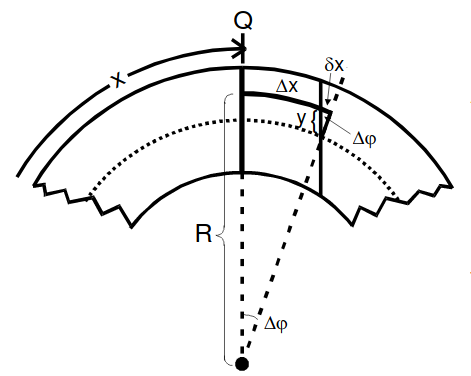
\includegraphics[scale=0.5]{Backfisch.png}
        \caption{Skizze zur Berechnung der Normalspannung $\sigma(y)$ in einem gebogenen Stab}
        \label{fig:backfisch}
    \end{figure}
    Aus geometrischen Günden, die in Abbildung \ref{fig:backfisch} ersichtlich sind, 
    ergibt sich für die Änderung $delta x$ einer Faser der Länge $\Delta x$
    \begin{equation*}
        \delta x = y \Delta \phi= y\dfrac{\Delta x}{R},
    \end{equation*}
    wobei y den Abstand der betrachteten zur neutralen Faser und R den Biegeradius
    symbolisiert. Anhand des Hookschen Gesetzes kann nun die durch die Biegung 
    entstehende Normalspannung bestimmt werden.
    \begin{equation*}
        \sigma(y)=E\dfrac{\delta x}{\Delta x}=E \dfrac{y}{R}
    \end{equation*}
    Auf einen Querschnitt Q wirken diese Spannungen wie ein Drehmoment $M_{\sigma}$ mit
    Hebelarm y. Das Geseamtdrehmoment, welches auf Querschnitt Q wirkt, lässt sich also 
    zu
    \begin{equation}
        \label{eqn:fuckyou}
        M_{\sigma}=\int_Q y \sigma(y)dq = \int_Q y^2 \dfrac{E}{R}dq 
    \end{equation}
    aufsummieren. 
    
\subsection{Biegung bei einseitiger Einspannung}
    \begin{figure}
        \centering
        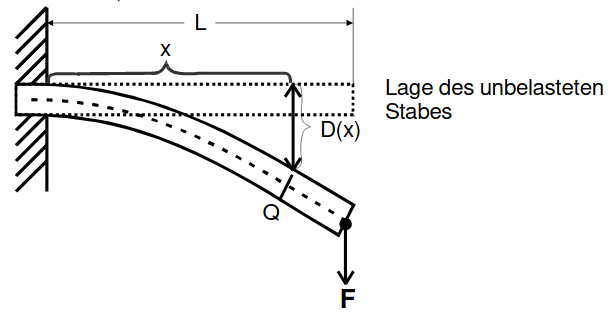
\includegraphics[scale=0.5]{Lebertransuppe.png}
        \caption{Durchbiegung eines elastischen Stabes bei einseitiger Einspannung}
        \label{fig:lebertran}
    \end{figure}
    Wird ein Stab einseitig eingespannt und ein Gewicht am uneingespannten Ende des Stabes 
    installiert, biegt sich der Stab aufgrund der Gravitation mit der Durchbiegung D(x) 
    und bewirkt am Ort x ein angreifendes Drehmoment
    \begin{equation}
        M_F = F \cdot (L − x)
    \end{equation}
    mit der Länge des Hebelarms (L − x). Dabei wird das Eigengewicht des Staber vernachlässigt.
    Dieses Drehmoment verursacht eine Biegung des Stabes, wodurch die im Kapitel 
    \ref{sec:aiaiai} berechneten Normalspannungen zustande kommen. Diese heben das 
    Drehmoment exakt auf, so dass ein Kräftegleichgewicht zwischen $M_F$ und $M_{\sigma}$ herrscht.
    \begin{equation}
        \int_Q y^2 \dfrac{E}{R}dq  = F \cdot (L − x)
    \end{equation}
    Der Krümmungsradius R kann durch $\dfrac{1}{R} \approx 
    \dfrac{d²D}{dx²}$ approximiert werden, sodass sich für Gleichung \ref{eqn:fuckyou}
    \begin{equation}
        E \dfrac{d²D}{dx²} \int_Q y² dq=F\cdot(L-x)
    \end{equation}
    ergibt. Die Durchbiegung kann also zu
    \begin{equation}
        D(x)=\dfrac{F}{2 E \ I}(Lx²-\dfrac{x^3}{3})
    \end{equation}
    mit Flächenträgheitsmoment
    \begin{equation}
        I = \int_Q y² dq
    \end{equation}
    bestimmt werden.

\subsection{Biegung bei zweiseitiger Auflage}
    \begin{figure}
        \centering
        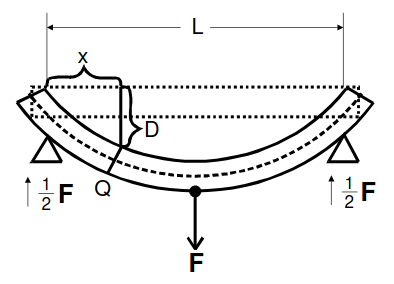
\includegraphics[scale=0.5]{Gemüsemedley.png}
        \caption{Durchbiegung eines elastischen Stabes bei beidseitiger Auflage}
        \label{fig:gemüse}
    \end{figure}
    Wie in Abb. \ref{fig:gemüse} dargestellt, wird bei beidseitiger Auflage ein Gewicht in der Mitte des 
    jeweiligen Stabes installiert, sodass dieser sich zur Mitte hin biegt. Bei dieser 
    Konstruktion greift am Ort x die Kraft $\dfrac{F}{2}$ mit Hebelarm x 
    beziehungsweise (L-x) auf der linken Seite an der Querschnittsfläche Q
    an. Auf die Querschnittsfläche wirkt also das Drehmoment $M_F = -\dfrac{F}{2} x$ 
    beziehungsweise $M_F = -\dfrac{F}{2}(L-x)$ auf der linken Seite des Stabes.
    Somit erhalten wir 
    \begin{equation}
        \text{für } 0 \leq x \leq \dfrac{L}{2}:\ \ \ \ \dfrac{d D}{dx}=-\dfrac{F}{E\ I}\dfrac{x^2}{4}+C \\
        \text{für} \dfrac{L}{2} \leq x \leq L:\ \ \ \ \dfrac{d D}{dx}=-\dfrac{F}{2 E\ I}(Lx - \dfrac{x^2}{2})+C'
    \end{equation}
    Da die Tangente in der Mitte des Stabes horizontal ist, gilt für 
    \begin{equation*}
        C = \dfrac{F}{E\ I}\dfrac{L^2}{16} \\
        C'=\dfrac{F}{E\ I}\dfrac{3L^2}{16}
    \end{equation*}
    Somit folgt für 
    \begin{align}
        \text{für } 0 \leq x \leq \dfrac{L}{2}\ \ \ \ D(x)=\dfrac{F}{48 E\ I}(3L^2x-4x^3) \\
        \text{für} \dfrac{L}{2} \leq x \leq L:\ \ \ \ D(x)=\dfrac{F}{48 E\ I}(4 x^3-12Lx^2+9L^2x-L^3) 
    \end{align}

%\subsection{Zusammenhang zwischen Elastizitätsmodul und Schallgeschwwindigkeit in Festkörpern}
%    Läuft eine Schallwelle durch einen Körper, so entsteht durch die longitudinale Deformation
%    Spannung. Ein Volumenelement $dV=Q\ dx$ an Ort x wird durch die Spannung $\sigma(x)$
%    um $\eta$ verschoben und um $d \eta$ degehnt, da an Ort x eine andere Spannung $\sigam(x)$
%    herrscht als bei x+dx, wo $\sigma(x)+d\sigma$ auftritt. Nach dem Hookschen Gesetz gilt:
%    \begin{equation*}
%        \sigma=E\dfrac{\partial \eta}{\partial x}
%    \end{equation*}
%    beziehungsweise
%    \begin{equation*}
%        \sigma + d \sigma = E \dfrac{\partial \eta}{\partial x}+E\dfrac{\partial^2 \eta}{\partial x^2}dx
%    \end{equation*}
%    Somit wirkt auf ein Volumenelement Q dx die Kraft
%    \begin{equation}
%        dF=Q((\sigma + d\sigma)-\sigma)=Q \ E\dfrac{\partial^2 \eta}{\partial x^2}dx
%    \end{equation}
%    Daraus lässt sich schlussfolgern, dass
%    \begin{equation}
%        \dfrac{\partial^2 \eta}{\partial t^2}=\dfrac{E}{\rho} \dfrac{\partial^2 \eta}{\partial x^2}
%    \end{equation}
%    Diese Wellengleichung schreibt der Ausbreitungsgeschwindigkeit $ c = \sqrt{\dfrac{E}{\rho}}$ zu.
%    Dies kann ebenfalls verwendet werden, um das Elastizitätsmodul E zu bestimmen.